% Presentación de tema · 20 min con preguntas (exposición prevista ~15 min).
% Orden = los cinco puntos del issue #7. Tiempos anotados por slide.
% Todo número económico sale de ../code/output/topic_numbers.tex (python code/verify.py).
\documentclass[aspectratio=169,11pt]{beamer}
\geometry{paperwidth=20cm,paperheight=11.25cm}
\usepackage[utf8]{inputenc}
\usepackage[T1]{fontenc}
\usepackage[spanish,es-nodecimaldot,es-noquoting]{babel}
\usepackage{lmodern,amsmath,amssymb,booktabs,array,tikz,colortbl}
\usetikzlibrary{arrows.meta,positioning,calc}
% Generated by python code/verify.py; do not edit numerical values by hand.
\newcommand{\PhiBase}{0.38}
\newcommand{\PhiMid}{0.50}
\newcommand{\PhiHigh}{0.70}
\newcommand{\PsiFormal}{55}
\newcommand{\PsiInformalBase}{34.00}
\newcommand{\PsiRecovered}{33.997018}
\newcommand{\PsiInformalHigh}{6.67}
\newcommand{\KappaBase}{0.4000}
\newcommand{\KappaHigh}{0.4029}
\newcommand{\TaxFormal}{0.18}
\newcommand{\NuInformal}{0.60}
\newcommand{\TimeCap}{1}
\newcommand{\MOnePercent}{51.71}
\newcommand{\MThreePP}{37.75}
\newcommand{\MThreePsiOnlyPP}{36.30}
\newcommand{\VThreeBasePP}{4.31}
\newcommand{\VThreeHighPP}{10.43}
\newcommand{\VThreeMatlabPP}{4.41}
\newcommand{\CapMassPercent}{0}
\newcommand{\MaxHoursBase}{0.75}
\newcommand{\MaxHoursHigh}{0.82}
\newcommand{\CentralProductivity}{0.8409}
\newcommand{\QOneMassPercent}{20.84}
\newcommand{\QOneMatlabMassPercent}{19.67}
\newcommand{\GridAssets}{200}
\newcommand{\GridProductivity}{40}
\newcommand{\VThreeThesisBasePP}{4.4}
\newcommand{\VThreeThesisHighPP}{10.6}
\newcommand{\QOneSharePercent}{54.3}
\newcommand{\QFiveSharePercent}{49.9}
\newcommand{\FocAPoor}{-0.2}
\newcommand{\FocARich}{12.3}
\newcommand{\FocPctFormal}{40}
\newcommand{\ShareCentralBase}{52}
\newcommand{\ShareHighPoor}{54}
\newcommand{\ShareHighRich}{47}
\newcommand{\FocPctInformalHigh}{86}
\newcommand{\IneiYear}{2017}
\newcommand{\GeAvailable}{0}
\newcommand{\GeVThreeBasePP}{4.4}
\newcommand{\GeMOneBase}{51.7}
\newcommand{\GeMThreeBase}{37.8}
\newcommand{\GeRBase}{6.60}
\newcommand{\GePIBase}{0.928}
\newcommand{\GeGiniBase}{0.521}
\newcommand{\GeSlopeBase}{0}
\newcommand{\GeVThreeMidPP}{--}
\newcommand{\GeMOneMid}{--}
\newcommand{\GeMThreeMid}{--}
\newcommand{\GeRMid}{--}
\newcommand{\GePIMid}{--}
\newcommand{\GeGiniMid}{--}
\newcommand{\GeSlopeMid}{--}
\newcommand{\GeVThreeHighPP}{--}
\newcommand{\GeMOneHigh}{--}
\newcommand{\GeMThreeHigh}{--}
\newcommand{\GeRHigh}{--}
\newcommand{\GePIHigh}{--}
\newcommand{\GeGiniHigh}{--}
\newcommand{\GeSlopeHigh}{--}
\newcommand{\GeKappaAvailable}{1}
\newcommand{\GeKappaVThreeRange}{4.37--4.39}
\newcommand{\GeVThreeBaseTwoPP}{4.41}
\newcommand{\VThreeNuOnePP}{2.3}
\newcommand{\KappaNuOne}{0.410}
\newcommand{\GiniAssets}{0.52}
\newcommand{\VThreeKappaRangeBase}{4.3--4.4}
\newcommand{\VThreeKappaRangeHigh}{10.5--10.6}
\newcommand{\KappaRangeShapes}{0.400--0.403}
\newcommand{\FrischFormalCR}{0.39}
\newcommand{\FrischInformalCR}{0.37}
\newcommand{\FrischGapCR}{$-$0.02}
\newcommand{\PhiEvidence}{0.36}
\newcommand{\VThreeEvidencePP}{4.0}
\newcommand{\KappaPercentile}{0.401}
\newcommand{\VThreePctBasePP}{4.4}
\newcommand{\VThreePctHighPP}{10.6}
\newcommand{\VSixData}{38.6}
\newcommand{\VSixModel}{6.2}
\newcommand{\VSixPercentile}{6.6}
\newcommand{\VSixAdValorem}{18.6}
\newcommand{\AdValoremMedianPercent}{94}
\newcommand{\AdValoremPsiI}{344}
\newcommand{\VThreeAdValoremPP}{13.0}
\newcommand{\VThreePercentilePP}{4.7}
\newcommand{\EduOddsData}{21}
\newcommand{\EduOddsModel}{1.6}
\newcommand{\EduRequiredRatio}{2\,926}
\newcommand{\ExtremeNodeMassPercent}{0.3}
\newcommand{\IneiQOne}{97.1}
\newcommand{\IneiQFive}{44.1}
\newcommand{\IneiQOneLatest}{94}
\newcommand{\IneiQFiveLatest}{49}
\newcommand{\IneiGapLatest}{44.7}
\newcommand{\IneiGapPreCovid}{52.6}
\newcommand{\DataMOne}{50.9}
\newcommand{\ModelMOne}{51.7}
\newcommand{\DataMTwo}{19.0}
\newcommand{\ModelMTwo}{18.8}
\newcommand{\DataMThree}{38.6}
\newcommand{\ModelMThree}{37.8}
\newcommand{\DataVOne}{2.30}
\newcommand{\ModelVOne}{2.33}
\newcommand{\DataVTwo}{1.913}
\newcommand{\ModelVTwo}{1.465}
\newcommand{\DataVThree}{53.0}
\newcommand{\ModelVThree}{4.4}
\newcommand{\DataVFour}{0.68}
\newcommand{\ModelVFour}{0.52}
\newcommand{\DataVFive}{0.40}
\newcommand{\ModelVFive}{0.22}
\newcommand{\CalibrationRows}{%
0.38 & 34.00 & 0.4000 & 4.41 \\
0.45 & 19.50 & 0.4008 & 5.77 \\
0.50 & 14.42 & 0.4013 & 6.75 \\
0.60 & 9.19 & 0.4022 & 8.68 \\
0.70 & 6.67 & 0.4029 & 10.59 \\
}

\usefonttheme{professionalfonts}

% ---------- Colores (los mismos de code/figures.py) ----------
\definecolor{Ink}{HTML}{172033}
\definecolor{Blue}{HTML}{223F91}
\definecolor{Teal}{HTML}{008A92}
\definecolor{Orange}{HTML}{D45D00}
\definecolor{Gray}{HTML}{5F6B7A}
\definecolor{Base}{HTML}{8A94A3}
\definecolor{Line}{HTML}{CCD4E2}
\definecolor{Pale}{HTML}{F3F5FA}
\definecolor{PaleTeal}{HTML}{EAF5F5}
\definecolor{PaleOrange}{HTML}{FDF1E6}
\setbeamercolor{normal text}{fg=Ink,bg=white}
\setbeamercolor{structure}{fg=Blue}
\setbeamercolor{frametitle}{fg=Ink,bg=white}
\setbeamercolor{alerted text}{fg=Orange}
\setbeamercolor{footleft}{fg=white,bg=Teal}
\setbeamercolor{footright}{fg=Gray,bg=Pale}
\setbeamerfont{frametitle}{size=\large,series=\bfseries}
\setbeamersize{text margin left=9mm,text margin right=9mm}
\setbeamertemplate{navigation symbols}{}
\setbeamertemplate{itemize items}[circle]
\setbeamertemplate{frametitle}{\vspace{1mm}\insertframetitle\par\vspace{1.5mm}{\color{Line}\hrule}\vspace{1mm}}
\hypersetup{pdftitle={Ahorro, flexibilidad de horas e informalidad en el Perú},pdfauthor={John Svante Barraza Ratachi},colorlinks=true,linkcolor=Ink,urlcolor=Blue}

% \textcolor starts the paragraph (\leavevmode): a bare \color at the top of a p{} cell shifts it down one line.
\newcommand{\teal}[1]{\textcolor{Teal}{#1}}
\newcommand{\orange}[1]{\textcolor{Orange}{#1}}
\newcommand{\gray}[1]{\textcolor{Gray}{#1}}
\newcommand{\labeltext}[1]{\par{\small\bfseries\color{Blue}#1\par}\vspace{1mm}}
\newcommand{\steplabel}[1]{\par{\small\bfseries\color{Teal}#1\par}\vspace{0.5mm}}
\newcommand{\panel}[3]{\begingroup\setlength{\fboxsep}{2.5mm}\colorbox{#1}{\begin{minipage}[t]{\dimexpr#2-5mm\relax}\raggedright #3\end{minipage}}\endgroup}
% Same as \panel with a fixed height, so panels side by side line up.
\newcommand{\panelh}[4]{\begingroup\setlength{\fboxsep}{2.5mm}\colorbox{#1}{\begin{minipage}[t][#3]{\dimexpr#2-5mm\relax}\raggedright #4\end{minipage}}\endgroup}
\newcommand{\takeaway}[1]{\par\vspace{3mm}\panel{PaleTeal}{\linewidth}{#1}\par}
\newcommand{\figurenote}[1]{\par\vspace{1mm}{\footnotesize\color{Gray}#1\par}}

% ---------- Barra superior con enlaces; pie de página con color ----------
\newcommand{\partid}{0}
\newcommand{\navitem}[3]{\hyperlink{#2}{\ifnum\partid=#1\textcolor{Teal}{\textbf{#3}}\else\textcolor{Gray}{#3}\fi}}
\setbeamertemplate{headline}{\vspace{2mm}\hspace{9mm}{\scriptsize
\navitem{1}{parte1}{1.\ Pregunta}\hspace{4mm}\navitem{2}{parte2}{2.\ Modelo y supuesto}\hspace{4mm}%
\navitem{3}{parte3}{3.\ Resultado esperado}\hspace{4mm}\navitem{4}{parte4}{4.\ Brecha en la literatura}\hspace{4mm}%
\navitem{5}{parte5}{5.\ Plan y riesgos}\hspace{4mm}\navitem{6}{anexos}{Anexos}}\par\vspace{0.5mm}}
\setbeamertemplate{footline}{\leavevmode\hbox{%
\begin{beamercolorbox}[wd=.42\paperwidth,ht=3.2ex,dp=1.3ex,leftskip=9mm]{footleft}\scriptsize\bfseries John Barraza · Track B\end{beamercolorbox}%
\begin{beamercolorbox}[wd=.58\paperwidth,ht=3.2ex,dp=1.3ex,rightskip=9mm]{footright}\scriptsize\hspace{4mm}Ahorro, flexibilidad de horas e informalidad en el Perú\hfill\insertframenumber/\inserttotalframenumber\end{beamercolorbox}}}

% Separador de parte: banda de color con el número y título a la derecha.
\newcommand{\separator}[5]{%
\renewcommand{\partid}{#1}
\begin{frame}[plain,label=#2]
\begin{tikzpicture}[remember picture,overlay]
\fill[#5] (current page.north west) rectangle ([xshift=62mm]current page.south west);
\node[white,font=\fontsize{64}{64}\selectfont\bfseries] at ([xshift=31mm]current page.west) {#3};
\node[anchor=west,text width=110mm,font=\LARGE\bfseries,text=Ink] at ([xshift=74mm,yshift=4mm]current page.west) {#4};
\draw[#5,line width=1.2pt] ([xshift=74mm,yshift=-6mm]current page.west) -- ++(110mm,0);
\end{tikzpicture}
\end{frame}}

\tikzset{
  agent/.style={draw=#1,line width=1.1pt,rounded corners=2pt,fill=white,align=center,inner sep=5pt},
  step/.style={draw=Line,line width=0.8pt,rounded corners=2pt,fill=Pale,align=center,inner sep=4pt,font=\small,text width=#1},
  flow/.style={-{Stealth[length=2.4mm]},line width=1pt,color=#1},
  flowlabel/.style={font=\small,align=center,fill=white,inner sep=1.5pt}
}

\begin{document}

% ===== Portada (0:20) =====
\begin{frame}[plain]
\begin{tikzpicture}[remember picture,overlay]
\fill[Teal] (current page.south west) rectangle ([yshift=4mm]current page.south east);
\end{tikzpicture}
\vspace{6mm}
{\small\bfseries\color{Blue}Universidad del Pacífico}\par
{\small AI and Economic Modeling · Track B: modelo económico de este trabajo}\par
\vspace{11mm}
{\LARGE\bfseries Ahorro, flexibilidad de horas\par\vspace{1.5mm}\teal{e informalidad en el Perú}\par}
\vspace{4mm}
{\large Riqueza y reparto de horas entre el sector formal y el informal en un modelo de agentes heterogéneos}\par
\vspace{9mm}
{\large John Svante Barraza Ratachi}\par
\vspace{1mm}
{\small Profesor: Alexander Quispe}\par
\vspace{8mm}
{\small\href{https://github.com/johnbarraza/ai-project}{github.com/johnbarraza/ai-project}\hfill Lima · 16 de octubre de 2026}
\end{frame}

% ===== Estructura (0:20) =====
\renewcommand{\partid}{0}
\begin{frame}{Estructura de la \teal{presentación}}
\vspace{2mm}
\renewcommand{\arraystretch}{1.9}
\begin{tabular}{@{}lll@{}}
\textcolor{Teal}{\textbf{1.}} & \hyperlink{parte1}{\textbf{Pregunta y track}} & \textcolor{Gray}{Un dato del Perú y la pregunta}\\
\textcolor{Teal}{\textbf{2.}} & \hyperlink{parte2}{\textbf{Modelo base y supuesto que cambio}} & \textcolor{Gray}{Aiyagari, mi modelo, equilibrio y momentos}\\
\textcolor{Teal}{\textbf{3.}} & \hyperlink{parte3}{\textbf{Resultado esperado}} & \textcolor{Gray}{FOC del hogar y conjetura, con gráficos}\\
\textcolor{Teal}{\textbf{4.}} & \hyperlink{parte4}{\textbf{Brecha en la literatura}} & \textcolor{Gray}{Aporte y pendiente de cada trabajo}\\
\textcolor{Teal}{\textbf{5.}} & \hyperlink{parte5}{\textbf{Plan y riesgos}} & \textcolor{Gray}{Demostración, simulación y formalización}\\
\textcolor{Orange}{\textbf{A}} & \hyperlink{anexos}{\textbf{Anexos}} & \textcolor{Gray}{Agentes, HJB/KF, mercados, parámetros, robustez, educación}\\
\end{tabular}
\end{frame}

% =====================================================================
\separator{1}{parte1}{1}{Pregunta y track}{Teal}

% ===== 1. Dato (1:00) =====
\renewcommand{\partid}{1}
\begin{frame}{1. El empleo informal es mayor \teal{en los quintiles de menor gasto}}
\centering
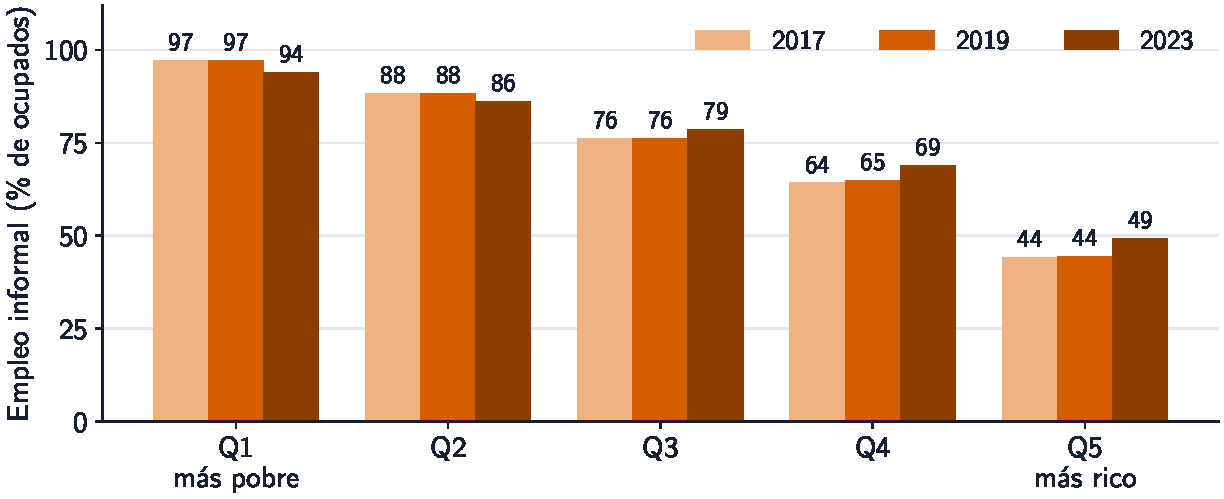
\includegraphics[width=\linewidth,height=5.5cm,keepaspectratio]{../code/figures/motivation_quintiles.pdf}
\takeaway{\small Este patrón motiva distinguir el papel de los activos del de la productividad laboral.}
\figurenote{Tasa de empleo informal de la población ocupada (empleo principal) por quintil de gasto per cápita del hogar, ENAHO.
Fuentes: INEI (2018, 2022); ENAHO 2023, elaboración propia.}
\end{frame}

% ===== 1. Pregunta (1:00) =====
\begin{frame}{1. La pregunta: \teal{riqueza y reparto de horas}}
\vfill
\panel{PaleTeal}{\linewidth}{\centering\vspace{3mm}
{\Large\bfseries ¿Cuándo influye la riqueza en el reparto de horas\par\vspace{1.5mm}
entre formal e informal, para una misma productividad?}\par\vspace{3mm}}
\vspace{8mm}
\begin{columns}[T,onlytextwidth]
\column{.47\textwidth}
\labeltext{Comparación}
El dato compara quintiles de gasto. El modelo compara activos para una misma productividad laboral individual, $z$.
\column{.47\textwidth}
\labeltext{Track B}
Modelo económico de \textit{Informalidad y distribución de riqueza en el Perú}.
\end{columns}
\vfill
\end{frame}

% =====================================================================
\separator{2}{parte2}{2}{Modelo base y supuesto que cambio}{Teal}

% ===== 2. Baseline (1:00) =====
\renewcommand{\partid}{2}
\begin{frame}{2. Baseline: \teal{Aiyagari (1994)}; el supuesto que cambio: \teal{dos sectores}}
\begin{tikzpicture}[card/.style={step=37mm,minimum height=24mm,font=\footnotesize,align=center,execute at begin node={\hyphenpenalty=10000\exhyphenpenalty=10000}}]
\node[card] (ai) at (0,0) {{\small\textbf{Aiyagari (1994)}}\\[1mm]Hogares que ahorran por precaución ante shocks de productividad. Una firma, un bien.};
\node[card] (ac) at (4.55,0) {{\small\textbf{Achdou et al. (2022)}}\\[1mm]El mismo modelo en tiempo continuo: decisiones (HJB) y distribución (KF).};
\node[card] (ga) at (9.1,0) {{\small\textbf{Galindo et al. (2024)}}\\[1mm]Aplicación al Perú: formales e informales como tipos exógenos; nadie elige.};
\node[card,draw=Teal,fill=PaleTeal] (me) at (13.65,0) {{\small\textbf{Modelo de dos sectores}}\\[1mm]Cada hogar reparte sus horas entre los dos sectores. Dos firmas y dos bienes.};
\draw[flow=Gray] (ai) -- (ac); \draw[flow=Gray] (ac) -- (ga); \draw[flow=Teal] (ga) -- (me);
\end{tikzpicture}
\vspace{5mm}
\begin{columns}[T,onlytextwidth]
\column{.47\textwidth}
\panel{Pale}{\linewidth}{\labeltext{Baseline: una firma y un bien}
\[
\max\ \mathbb E_0\!\int_0^\infty e^{-\rho t}u(c_t)\,dt
\quad\text{s.a.}\quad \dot a=wz+ra-c
\]
{\footnotesize\gray{$u$: utilidad; $\rho$: descuento; $w$: salario; límite de deuda $a\ge\underline a$.}}\par\vspace{1.5mm}
\textbf{Equilibrio:} ahorro $=$ capital ($A=K$) fija $r$.}
\column{.47\textwidth}
\panel{PaleTeal}{\linewidth}{\labeltext{Modelo de dos sectores}
Horas endógenas en dos sectores: $\ell_F$ y $\ell_I$.\par
Dos firmas y dos bienes: precios $r$ y $p_I$.\par
Barrera $\kappa(z)$ y prima de deuda $\chi(z)$.\par
\gray{Con un solo sector vuelve a Aiyagari.}}
\end{columns}
\end{frame}

% ===== 2. Agentes (0:45) =====
\begin{frame}{2. Modelo de dos sectores: \teal{hogares, dos firmas y un gobierno}}
\centering
\vspace{2mm}
\begin{tikzpicture}[x=1cm,y=1cm]
\node[agent=Teal,text width=32mm,minimum height=50mm,font=\normalsize] (H) at (0,0) {\textbf{Hogares}\\[2mm]\small activos $a$\\ productividad $z$\\[2mm]\footnotesize eligen consumo\\ y horas};
\node[agent=Orange,text width=40mm,minimum height=18mm,font=\normalsize] (FI) at (9.2,1.6) {\textbf{Firma informal}\\\small bien informal, precio $p_I$};
\node[agent=Blue,text width=40mm,minimum height=18mm,font=\normalsize] (FF) at (9.2,-1.6) {\textbf{Firma formal}\\\small bien formal, precio 1};
\node[agent=Gray,text width=32mm,font=\normalsize] (G) at (0,-3.65) {\textbf{Gobierno}};
\draw[flow=Orange] (1.85,1.95) -- node[flowlabel,above]{horas $\ell_I$, ahorro} (6.9,1.95);
\draw[flow=Orange] (6.9,1.25) -- node[flowlabel,below,text width=44mm]{ingreso $R_I(z)$ por hora, bien $c_I$} (1.85,1.25);
\draw[flow=Blue] (1.85,-1.25) -- node[flowlabel,above]{horas $\ell_F$, ahorro} (6.9,-1.25);
\draw[flow=Blue] (6.9,-1.95) -- node[flowlabel,below,text width=44mm]{salario neto $R_F(z)$ por hora,\\ bien $c_F$} (1.85,-1.95);
\draw[flow=Gray] (-0.6,-2.55) -- node[flowlabel,left]{impuesto $\tau$} (-0.6,-3.35);
\draw[flow=Gray] (0.6,-3.35) -- node[flowlabel,right]{transferencia $T$} (0.6,-2.55);
\end{tikzpicture}
\figurenote{Todos toman los precios como dados; el equilibrio los determina. Quién elige qué: \hyperlink{a1}{anexo A1}; variables: \hyperlink{avar}{anexo A2}; firmas: \hyperlink{afirm}{anexo A4}.}
\end{frame}

% ===== 2. Timing (0:45) =====
\begin{frame}{2. En cada instante el hogar \teal{observa, decide y su estado cambia}}
\centering
\vspace{3mm}
\begin{tikzpicture}[node distance=7mm,every node/.append style={minimum height=19mm}]
\node[step=31mm] (s1) {\textbf{1. Observa}\\ activos $a$ y\\ productividad $z$};
\node[step=31mm,right=of s1] (s2) {\textbf{2. Decide}\\ consumo $c_F,c_I$\\ horas $\ell_F,\ell_I$};
\node[step=31mm,right=of s2,fill=PaleOrange] (s3) {\textbf{3. Evolucionan}\\ $a$: ahorro\\ $z$: azar exógeno};
\node[step=31mm,right=of s3] (s4) {\textbf{4. Reoptimiza}\\ observa el nuevo\\ estado $(a,z)$};
\draw[flow=Ink] (s1) -- (s2); \draw[flow=Ink] (s2) -- (s3); \draw[flow=Ink] (s3) -- (s4);
\draw[flow=Teal] (s4.south) -- ++(0,-6mm) -| node[flowlabel,minimum height=0pt,pos=0.25]{\teal{decisiones que se actualizan en tiempo continuo}} (s1.south);
\end{tikzpicture}
\vspace{6mm}
\begin{columns}[T,onlytextwidth]
\column{.47\textwidth}
\panel{PaleOrange}{\linewidth}{\textbf{Sabe:} su $z$ actual y cómo puede cambiar.\par\vspace{1mm}
\textbf{No sabe:} la realización futura del choque. La persistencia no elimina la incertidumbre.}
\column{.47\textwidth}
\panel{Pale}{\linewidth}{\textbf{Estado estacionario:} la distribución $g(a,z)$ no cambia, aunque cada hogar sigue moviéndose dentro de ella.}
\end{columns}
\end{frame}

% ===== 2. Hogar (1:15) =====
\begin{frame}{2. El \teal{hogar} maximiza su utilidad sujeto a recursos y tiempo}
\panel{PaleTeal}{\linewidth}{\labeltext{\color{Teal}Objetivo}
\[
\max_{c_F,\,c_I,\,\ell_F,\,\ell_I}\ \ \mathbb E_0\int_0^\infty e^{-\rho t}
\Big[\ln C-\frac{\psi_F\,\ell_F^{1+1/\phi_F}}{1+1/\phi_F}-\frac{\psi_I\,\ell_I^{1+1/\phi_I}}{1+1/\phi_I}\Big]dt
\]}
\labeltext{Restricciones}
\[
\dot a=\underbrace{R_F(z)\ell_F+R_I(z)\ell_I}_{\text{ingreso laboral}}+ra-\chi(z)\max(-a,0)+T-c_F-p_Ic_I,
\qquad a\ge\underline a,\qquad \ell_F+\ell_I\le\bar H
\]
\vspace{1mm}
\footnotesize
\begin{columns}[T,onlytextwidth]
\column{.48\textwidth}
$C$: canasta CES de $c_F$ y $c_I$; $\rho$: descuento.\par
$\psi_s$: desutilidad del trabajo en $s$; $\phi_s$: elasticidad de esas horas.
\column{.48\textwidth}
$\chi(z)\max(-a,0)$: prima sobre la deuda. Con $a<0$ paga $r+\chi(z)$ por sol debido; con $a\ge0$ el término es cero. $\underline a$: límite de deuda.\par
$\bar H$: tiempo disponible; $R_F$, $R_I$: ingreso por hora en cada sector.
\end{columns}
\end{frame}

% ===== 2. Ingreso por hora y barrera (1:00) =====
\begin{frame}{2. La barrera y la prima de deuda \teal{caen con la productividad}}
\begin{columns}[T,onlytextwidth]
\column{.48\textwidth}
\panel{Pale}{\linewidth}{\labeltext{Ingreso por hora que recibe el hogar}
\[
R_F(z)=(1-\tau)\,w_F\,z-\kappa(z)
\]
\[
R_I(z)=\widetilde w_I\,z^{\nu_I}
\]}
\column{.48\textwidth}
\panel{PaleTeal}{\linewidth}{\labeltext{\color{Teal}Una misma escala para las dos cuñas}
\[
\kappa(z)=\kappa_{z1}\,w(z),\qquad \chi(z)=\chi\,w(z)^{\eta}
\]
\[
w(z)=\frac{z_{\max}-z}{z_{\max}-z_{\min}}\in[0,1]
\]}
\end{columns}
\vspace{3mm}
\small
\renewcommand{\arraystretch}{1.35}
\begin{tabular}{@{}>{\raggedright\arraybackslash}p{24mm}>{\raggedright\arraybackslash}p{58mm}@{\hspace{8mm}}>{\raggedright\arraybackslash}p{24mm}>{\raggedright\arraybackslash}p{58mm}@{}}
$\tau$ & impuesto al ingreso laboral formal & $w(z)$ & índice que disminuye con la productividad\\
$\widetilde w_I$ & pago informal por trabajo efectivo & $\kappa_{z1}$ & barrera formal máxima por hora\\
$\nu_I$ & cómo influye $z$ en el ingreso informal por hora & $\chi,\ \eta$ & escala y forma de la prima de deuda\\
\end{tabular}\par
\vspace{2mm}
{\footnotesize\color{Gray}Valores y fuentes: \hyperlink{a5}{anexo A8}. Formas alternativas: \hyperlink{aforms}{anexo A12}.}
\end{frame}

% ===== 2. Informalidad por productividad (0:50) =====
\begin{frame}{2. En el modelo de dos sectores, \teal{la informalidad cae con la productividad}}
\centering
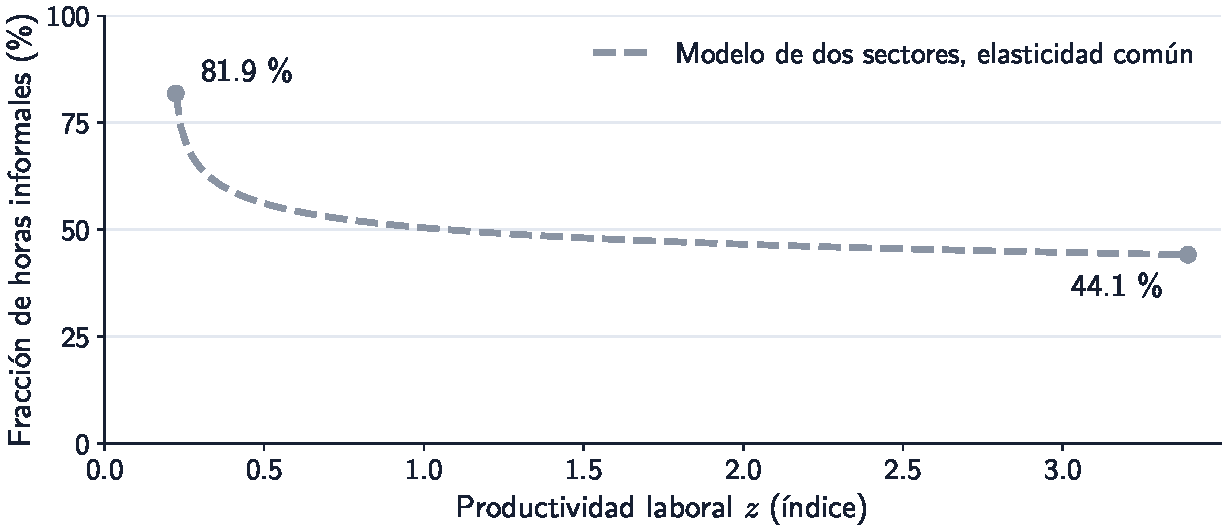
\includegraphics[width=.98\linewidth,height=5.7cm,keepaspectratio]{../code/figures/informal_share_by_productivity.pdf}
\takeaway{\small La productividad es exógena; el hogar elige cómo repartir sus horas.}
\figurenote{Solución estacionaria del modelo de dos sectores, $\phi_F=\phi_I=\PhiBase$. Mercado de activos: \hyperlink{aasset}{anexo A16}.}
\end{frame}

% ===== 2. Supuesto que cambio (1:15) =====
\begin{frame}{2. Sensibilidad: \teal{elasticidades distintas}}
\vfill
\begin{columns}[T,onlytextwidth]
\column{.47\textwidth}
\panelh{Pale}{\linewidth}{40mm}{\labeltext{\color{Gray}Modelo de dos sectores}
\[
\phi_F=\phi_I=\PhiBase
\]
Ambas horas responden igual a $V_a$.\par\vspace{2mm}
A igual productividad, la riqueza no mueve la proporción informal.}
\column{.47\textwidth}
\panelh{PaleTeal}{\linewidth}{40mm}{\labeltext{\color{Teal}Sensibilidad}
\[
\phi_I\in[\PhiBase,\PhiHigh],\qquad\phi_F=\PhiBase
\]
Permito una mayor respuesta de las horas informales.\par\vspace{2mm}
Examino cuánto depende el reparto de horas de haber impuesto elasticidades iguales.}
\end{columns}
\takeaway{\small Comparación parcial: precios, $V_a$ y distribución fijos. Recalibro para conservar M1 y M3. El rango es una sensibilidad, no una estimación.}
\vspace{2mm}
{\color{Line}\rule{0.35\linewidth}{0.4pt}}\par\vspace{1mm}
{\footnotesize\color{Gray}$\phi_s$: elasticidad de Frisch, cuánto suben (\%) las horas en $s$ si el beneficio de una hora más sube 1\,\%.\par}
\end{frame}

% =====================================================================
\separator{3}{parte3}{3}{Resultado esperado}{Teal}

% ===== 3. FOC (1:30) =====
\renewcommand{\partid}{3}
\begin{frame}{3. FOC del hogar: \teal{el beneficio de una hora más iguala su costo}}
\panel{Pale}{\linewidth}{\steplabel{1. Parto de la HJB del hogar (\hyperlink{a2}{anexo A3})}
\vspace{-2mm}\[
\rho v(a,z)=\max_{c_F,c_I,\ell_F,\ell_I}\Big\{\ln C-\sum_{s}\frac{\psi_s\ell_s^{1+1/\phi_s}}{1+1/\phi_s}+V_a\,\dot a\Big\}+\sum_{z'}\lambda_{zz'}\big[v(a,z')-v(a,z)\big]
\]
\vspace{1mm}{\small $V_a=\partial v/\partial a$: valor marginal de los activos.}}
\vspace{2mm}
\begin{columns}[T,onlytextwidth]
\column{.315\textwidth}
\panelh{Pale}{\linewidth}{26mm}{\steplabel{2. Bloque de horas}
\vspace{-1mm}\[
\max_{\ell_s\ge0}\ V_aR_s\ell_s-\frac{\psi_s\ell_s^{1+1/\phi_s}}{1+1/\phi_s}
\]
\footnotesize con $V_a$ y precios dados}
\column{.315\textwidth}
\panelh{Pale}{\linewidth}{26mm}{\steplabel{3. Derivo respecto de $\ell_s$}
\vspace{-1mm}\[
V_aR_s(z)-\psi_s\ell_s^{1/\phi_s}
\]
\footnotesize beneficio menos costo de una hora más}
\column{.315\textwidth}
\panelh{PaleTeal}{\linewidth}{26mm}{\steplabel{4. Igualo a cero}
\vspace{-1mm}\[
\boxed{V_aR_s(z)=\psi_s\ell_s^{1/\phi_s}}
\]
\footnotesize BMg $=$ CMg $\Rightarrow\ \ell_s=(V_aR_s/\psi_s)^{\phi_s}$}
\end{columns}
\takeaway{\small\textbf{A igual productividad y retornos dados:} mayor $V_a$ implica más horas en \emph{ambos} sectores.
En equilibrio general cambian retornos, $V_a$ y distribución; estas FOC no fijan el efecto final.}
\figurenote{Vale con solución interior, $\ell_F+\ell_I<\bar H$: en el modelo de dos sectores el máximo es $\MaxHoursBase$ con $\bar H=\TimeCap$. Con tope de tiempo: \hyperlink{a4}{anexo A7}.}
\end{frame}

% ===== 3. FOC gráfica (1:00) =====
\begin{frame}{3. La misma diferencia de $V_a$ \teal{mueve más las horas informales}}
\centering
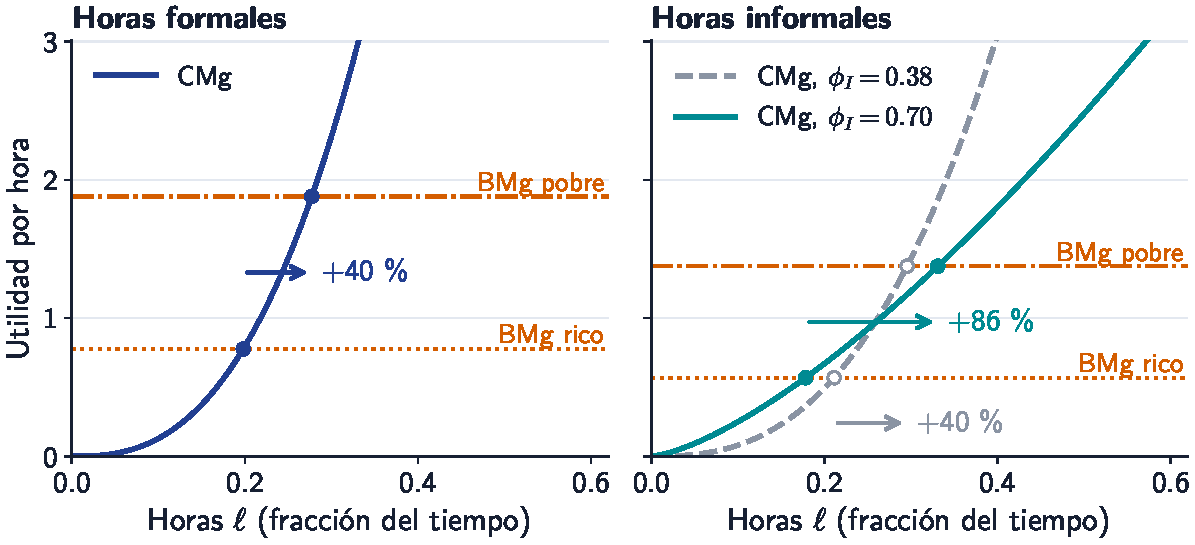
\includegraphics[width=\linewidth,height=6.3cm,keepaspectratio]{../code/figures/foc_hours.pdf}
\figurenote{Calibrado, equilibrio parcial; mismo $z=\CentralProductivity$, pobre en el percentil 10 de riqueza y rico en el 90.
Rectas: BMg $=V_aR_s(z)$, una por hogar. Curvas: CMg $=\psi_s\ell^{1/\phi_s}$. Cada corte son las horas óptimas.}
\end{frame}

% ===== 3. Conjetura (2:00) =====
\begin{frame}{3. Conjetura: \teal{la riqueza cambia la composición de horas}}
\vfill
\[
\frac{\ell_I}{\ell_F}\;\propto\;V_a^{\,\phi_I-\phi_F}
\]
\vspace{8mm}
\panel{PaleTeal}{\linewidth}{\large
Si $\phi_I>\phi_F$ y $V_a$ disminuye con los activos, menos activos implican una mayor fracción de horas informales, a igual productividad.}
\par\vspace{5mm}
{\small Resultado condicionado: \hyperlink{aresult}{definiciones y condiciones completas en el anexo A17}.}
\vfill
\end{frame}

% ===== 3. Gráfico por activos (1:00) =====
\begin{frame}{3. Con $\phi_I>\phi_F$ la fracción informal \teal{cae con los activos}}
\centering
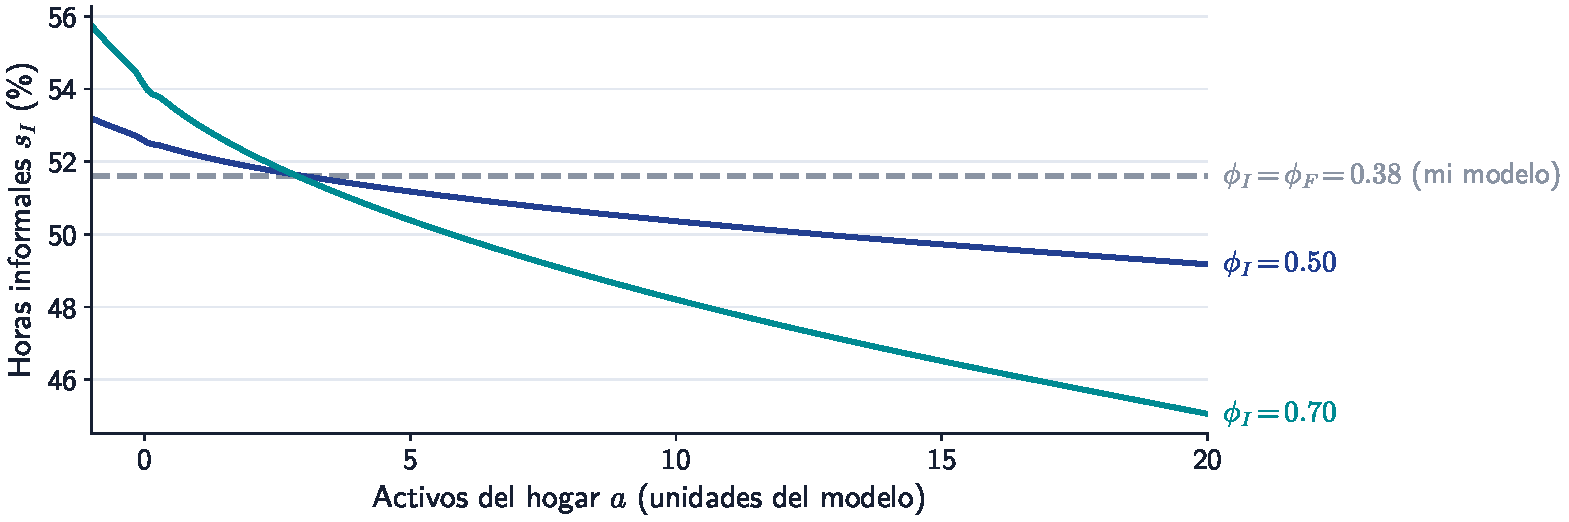
\includegraphics[width=\linewidth,height=6.4cm,keepaspectratio]{../code/figures/informal_share_by_assets.pdf}
\figurenote{Calibrado, equilibrio parcial: $V_a$, $g$ y precios del modelo de dos sectores. Mismo $z=\CentralProductivity$.
Línea gris: modelo de dos sectores ($\phi_I=\phi_F=\PhiBase$), plana porque $V_a$ se cancela. Cada curva recalibra $\psi_I$ y $\kappa_{z1}$ para mantener M1 y M3.}
\end{frame}

% =====================================================================
\separator{4}{parte4}{4}{Brecha en la literatura}{Teal}

% ===== 4. Literatura (1:30) =====
\renewcommand{\partid}{4}
\begin{frame}{4. Mi pregunta: \teal{riqueza y reparto elegido de horas}}
\footnotesize
\renewcommand{\arraystretch}{1.18}
\begin{tabular}{@{}>{\raggedright\arraybackslash}p{44mm}>{\raggedright\arraybackslash}p{60mm}>{\raggedright\arraybackslash}p{56mm}@{}}
\toprule
\textbf{Trabajo} & \textbf{Aporte} & \textbf{Pendiente para mi pregunta}\\
\midrule
\href{https://doi.org/10.2307/2118417}{Aiyagari (1994)}; \href{https://doi.org/10.1016/0165-1889(93)90024-M}{Huggett (1993)} & Ahorro precautorio con mercados incompletos & Un sector; horas fijas\\
\href{https://doi.org/10.1016/j.red.2005.11.002}{Pijoan-Mas (2006)} & Oferta laboral endógena: trabajar más horas también asegura & Un sector: no hay reparto\\
\href{https://doi.org/10.1093/restud/rdab002}{Achdou et al. (2022)} & Tiempo continuo: HJB y KF & Un sector\\
\href{https://doi.org/10.1596/978-0-8213-7092-6}{Perry et al. (2007)}; \href{https://doi.org/10.1111/twec.12480}{Loayza (2016)} & Informalidad por exclusión o por decisión & Sin distribución de riqueza\\
\href{https://doi.org/10.1257/aer.20121110}{Meghir, Narita y Robin (2015)} & Búsqueda de empleo formal e informal & Sin ahorro\\
\href{https://ideas.repec.org/p/rbp/wpaper/2024-005.html}{Galindo et al. (2024)} & Informalidad y riqueza en el Perú, con ingreso exógeno & Tipos exógenos (cambian al azar): nadie elige ni reparte horas\\
\bottomrule
\end{tabular}
\takeaway{\small Galindo et al. ya conectan informalidad y distribución de riqueza, pero con el sector exógeno. Aquí el hogar elige el reparto, y pregunto cuándo la riqueza lo mueve.}
\end{frame}

% =====================================================================
\separator{5}{parte5}{5}{Plan y riesgos}{Teal}

% ===== 5. Plan (1:15) =====
\renewcommand{\partid}{5}
\begin{frame}{5. Del resultado condicional \teal{al equilibrio general}}
\begin{columns}[T,onlytextwidth]
\column{.31\textwidth}
\panel{Pale}{\linewidth}{\labeltext{Demostrar}
La pendiente de $s_I$ en $V_a$ con sus tres condiciones, a mano y con verificación simbólica.}
\column{.31\textwidth}
\panel{Pale}{\linewidth}{\labeltext{Simular}
Equilibrio general con $\phi_I\neq\phi_F$ en el solver del modelo de dos sectores: ¿sobrevive la pendiente cuando cambian $r$, $p_I$ y $V_a$?}
\column{.31\textwidth}
\panel{Pale}{\linewidth}{\labeltext{Formalizar en Lean}
La proposición condicional, con AppliedModelingLib sobre el paper final.}
\end{columns}
\vspace{4mm}
\panel{PaleTeal}{\linewidth}{\labeltext{\color{Teal}Estimar $\phi_I$}
En el modelo, a igual $z$, las horas solo varían por $V_a$:
$\ \mathrm{sd}(\ln\ell_I\mid z)\,/\,\mathrm{sd}(\ln\ell_F\mid z)=\phi_I/\phi_F$. Se mide con ENAHO dentro de cada nivel educativo.}
\vspace{2mm}
\panel{PaleOrange}{\linewidth}{\labeltext{\color{Orange}Paso más riesgoso}
En equilibrio general cambian $r$, $p_I$ y la distribución: la brecha podría ser menor.
Primer intento: el solver reproduce el modelo de dos sectores, pero con $\phi_I=\PhiMid$ y $\PhiHigh$ aún no converge.
\textbf{Plan B:} el resultado condicional y el experimento parcial como cota.}
\end{frame}

% ===== 5. Cierre (0:30) =====
\begin{frame}{5. La respuesta \teal{que busco}}
\vfill
\panel{PaleTeal}{\linewidth}{\large
Bajo las condiciones de la conjetura, la riqueza influye en el reparto cuando las elasticidades son distintas.\par\vspace{4mm}
$\phi_I=\phi_F$: la riqueza no cambia la fracción informal.\par\vspace{3mm}
$\phi_I>\phi_F$: menos activos, mayor fracción informal.\par\vspace{3mm}
$\phi_I<\phi_F$: menos activos, menor fracción informal.}\par
\vfill
\end{frame}

% =====================================================================
\renewcommand{\partid}{6}
\begin{frame}[plain,label=anexos]
\centering
\vfill
{\fontsize{38}{44}\selectfont\bfseries\color{Teal}ANEXOS\par}
\vfill
\end{frame}

\begin{frame}[label=anexosindice]{\orange{Índice de anexos}}
\vfill
\renewcommand{\arraystretch}{1.65}
\begin{columns}[T,onlytextwidth]
\column{.48\textwidth}
\begin{tabular}{@{}l@{\hspace{2mm}}p{67mm}@{}}
\textcolor{Orange}{\textbf{A1}} & \hyperlink{a1}{Decisiones y precios dados}\\
\textcolor{Orange}{\textbf{A2}} & \hyperlink{avar}{Variables y estados}\\
\textcolor{Orange}{\textbf{A3}} & \hyperlink{a2}{Dinámica del hogar y distribución}\\
\textcolor{Orange}{\textbf{A4}} & \hyperlink{afirm}{Firmas y demanda de factores}\\
\textcolor{Orange}{\textbf{A5}} & \hyperlink{aeq}{Bucle de equilibrio}\\
\textcolor{Orange}{\textbf{A6}} & \hyperlink{a3}{Agregación y mercados}\\
\textcolor{Orange}{\textbf{A7}} & \hyperlink{a4}{Restricción de tiempo}\\
\textcolor{Orange}{\textbf{A8}} & \hyperlink{a5}{Parámetros y fuentes}\\
\textcolor{Orange}{\textbf{A9}} & \hyperlink{amom}{Metas y validaciones}\\
\end{tabular}
\column{.48\textwidth}
\begin{tabular}{@{}l@{\hspace{2mm}}p{67mm}@{}}
\textcolor{Orange}{\textbf{A10}} & \hyperlink{a6}{Recalibración de momentos}\\
\textcolor{Orange}{\textbf{A11}} & \hyperlink{av3}{Brecha Q1$-$Q5 y elasticidad}\\
\textcolor{Orange}{\textbf{A12}} & \hyperlink{aforms}{Formas de barrera y deuda}\\
\textcolor{Orange}{\textbf{A13}} & \hyperlink{a7}{Robustez de los resultados}\\
\textcolor{Orange}{\textbf{A14}} & \hyperlink{a8}{Formalidad por educación}\\
\textcolor{Orange}{\textbf{A15}} & \hyperlink{a9}{Referencias y datos}\\
\textcolor{Orange}{\textbf{A16}} & \hyperlink{aasset}{Mercado de activos}\\
\textcolor{Orange}{\textbf{A17}} & \hyperlink{aresult}{Conjetura: definiciones y condiciones}\\
\end{tabular}
\end{columns}
\vfill
\end{frame}

% ===== A1 =====
\begin{frame}[label=a1]{A1. Decisiones de cada agente y \teal{precios que toma dados}}
\renewcommand{\arraystretch}{1.4}
\begin{tabular}{@{}p{38mm}p{58mm}p{66mm}@{}}
\toprule
\textbf{Agente} & \textbf{Elige} & \textbf{Toma como dado}\\
\midrule
Hogar & $c_F,\ c_I,\ \ell_F,\ \ell_I$ (y así su ahorro) & $r,\ p_I,\ w_F,\ \widetilde w_I,\ T$ y su estado $(a,z)$\\
Firma formal & $K_F,\ L_F$ & $r,\ w_F$\\
Firma informal & $K_I,\ L_I$ & $r,\ p_I,\ w_I$\\
Gobierno & nada: sigue una regla & $T=\tau w_FL_F$\\
\bottomrule
\end{tabular}\par
\vspace{5mm}
Nadie elige los precios: $r$ y $p_I$ se ajustan hasta cerrar los mercados de activos y del bien informal; $w_F$ y $w_I$ salen de las FOC de las firmas.
\end{frame}

% ===== Anexo: variables =====
\begin{frame}[label=avar]{A2. Variables: \teal{estado}, \teal{decisiones} y \orange{precios}}
\small
\renewcommand{\arraystretch}{1.3}
\begin{tabular}{@{}p{33mm}p{35mm}p{98mm}@{}}
\toprule
\textbf{Tipo} & \textbf{Símbolo} & \textbf{Significado}\\
\midrule
\teal{Estado del hogar} & $a$ & activos; \textbf{endógeno}: lo mueve el ahorro\\
 & $z$ & productividad laboral; \textbf{exógena}: proceso OU en $\ln z$\\
\teal{Decisiones del hogar} & $c_F,\ c_I$ & consumo de bien formal e informal\\
 & $\ell_F,\ \ell_I$ & horas formales e informales, con $\ell_F+\ell_I\le\bar H$\\
\teal{Decisiones de firmas} & $K_s,\ L_s$ & capital y trabajo efectivo de cada sector $s\in\{F,I\}$\\
\orange{Precios de equilibrio} & $r,\ p_I$ & interés y precio del bien informal: \textbf{se ajustan} hasta cerrar los mercados\\
 & $w_F,\ w_I,\ T$ & salen de las FOC de las firmas y de la regla del gobierno\\
\gray{Objetos de solución} & $v(a,z),\ V_a$ & valor del hogar y valor de un sol más de activos, $V_a=\partial v/\partial a$\\
 & $g(a,z)$ & distribución de hogares\\
\bottomrule
\end{tabular}
\end{frame}

% ===== A2 =====
\begin{frame}[label=a2]{A3. Problema dinámico del hogar y \teal{distribución estacionaria}}
\labeltext{La productividad es exógena: proceso OU en logaritmos}
\[
d\ln z=-\eta_z\,(\ln z-\mu)\,dt+\sigma\,dW,\qquad\text{discretizado en }N_z=\GridProductivity\text{ nodos}
\]
\labeltext{HJB: valor del hogar dados los precios}
\[
\rho\,v(a,z)=\max_{c_F,c_I,\ell_F,\ell_I}\Big\{\ln C-\sum_{s}\frac{\psi_s\ell_s^{1+1/\phi_s}}{1+1/\phi_s}+V_a\,\dot a\Big\}
+\sum_{z'}\lambda_{zz'}\big[v(a,z')-v(a,z)\big]
\]
\labeltext{KF: la distribución no cambia en el estado estacionario}
\[
0=-\partial_a\big[\dot a(a,z)\,g(a,z)\big]+\sum_{z'}\big[\lambda_{z'z}\,g(a,z')-\lambda_{zz'}\,g(a,z)\big],\qquad \textstyle\sum_z\int g\,da=1
\]
\footnotesize $\lambda_{zz'}$: intensidad con que $z$ salta al nodo $z'$ (discretización del OU). La FOC de horas sale de derivar la llave $\{\cdot\}$ respecto de $\ell_s$; $\dot a$ es la restricción presupuestaria.
Grilla: $\GridAssets$ nodos de activos por $\GridProductivity$ de productividad.
\end{frame}

% ===== Anexo: firmas =====
\begin{frame}[label=afirm]{A4. Cada \teal{firma} contrata capital y trabajo hasta igualar su costo}
\begin{columns}[T,onlytextwidth]
\column{.48\textwidth}
\panel{Pale}{\linewidth}{\labeltext{\color{Blue}Firma formal: rendimientos constantes}
\[
\max_{K_F,L_F}\ A_FK_F^{\alpha}L_F^{1-\alpha}-w_FL_F-(r+\delta)K_F
\]
\textbf{FOC:}
\[
\underbrace{\alpha\frac{Y_F}{K_F}=r+\delta}_{\text{capital}},\qquad
\underbrace{(1-\alpha)\frac{Y_F}{L_F}=w_F}_{\text{trabajo}}
\]
Beneficio cero: los pagos agotan el producto.}
\column{.48\textwidth}
\panel{PaleOrange}{\linewidth}{\labeltext{\color{Orange}Firma informal: rendimientos decrecientes}
\[
\max_{K_I,L_I}\ p_IA_IK_I^{\alpha_I}L_I^{\beta_I}-w_IL_I-(r+\delta)K_I
\]
\textbf{FOC:}
\[
\underbrace{\alpha_I\frac{p_IY_I}{K_I}=r+\delta}_{\text{capital}},\qquad
\underbrace{\beta_I\frac{p_IY_I}{L_I}=w_I}_{\text{trabajo}}
\]
Con $\alpha_I+\beta_I<1$ queda un beneficio $\Pi_I>0$.}
\end{columns}
\vspace{3mm}
{\footnotesize $L_s$: trabajo efectivo, la suma de $z\,\ell_F$ (formal) o de $z^{\nu_I}\ell_I$ (informal) de los hogares.
El beneficio informal se reparte por hora efectiva: $\widetilde w_I=w_I+\Pi_I/L_I$.}
\end{frame}

% ===== Anexo: equilibrio =====
\begin{frame}[label=aeq]{A5. El equilibrio: \teal{$r$ y $p_I$ se ajustan} hasta que los mercados cierran}
\centering
\vspace{4mm}
\begin{tikzpicture}[node distance=6mm]
\node[step=27mm,fill=PaleOrange] (p) {\textbf{Precios}\\ $r,\ p_I$};
\node[step=33mm,right=of p] (d) {\textbf{Decisiones}\\ firmas: FOC $\to w_F,w_I$\\ hogares: HJB $\to c,\ell$};
\node[step=27mm,right=of d] (g) {\textbf{Distribución}\\ $g(a,z)$ con KF};
\node[step=35mm,right=of g] (m) {\textbf{¿Cierran?}\\ ahorro $=K_F+K_I$\\ $C_I=Y_I$};
\draw[flow=Ink] (p) -- (d); \draw[flow=Ink] (d) -- (g); \draw[flow=Ink] (g) -- (m);
\draw[flow=Orange] (m.south) -- ++(0,-7mm) -| node[flowlabel,pos=0.25]{\orange{no: subir o bajar $r$ y $p_I$ y repetir}} (p.south);
\draw[flow=Teal] (m.north) -- ++(0,6mm) node[above,font=\small,Teal]{sí: equilibrio};
\end{tikzpicture}
\vspace{6mm}
\begin{columns}[T,onlytextwidth]
\column{.47\textwidth}
\panel{Pale}{\linewidth}{\textbf{Activos} $\to r$: el ahorro de los hogares financia el capital de ambas firmas.\par\vspace{1mm}
\textbf{Bien informal} $\to p_I$: el consumo iguala la producción informal. El bien formal cierra por Walras (\hyperlink{a3}{anexo A6}).}
\column{.47\textwidth}
\panel{PaleOrange}{\linewidth}{\textbf{En este proyecto, por ahora:} equilibrio \emph{parcial}.
Fijo precios, $V_a$ y $g$ en los del modelo de dos sectores y cambio solo el bloque de horas.}
\end{columns}
\end{frame}

% ===== A3 =====
\begin{frame}[label=a3]{A6. Agregación y \teal{vaciado de mercados}}
\begin{columns}[T,onlytextwidth]
\column{.48\textwidth}
\labeltext{Sumo sobre hogares}
\[
S=\textstyle\sum_z\int a\,g\,da,\qquad L_F=\sum_z\int z\,\ell_F\,g\,da
\]
\[
L_I=\textstyle\sum_z\int z^{\nu_I}\ell_I\,g\,da,\qquad C_I=\sum_z\int c_I\,g\,da
\]
\labeltext{Gobierno}
\[
T=\tau\,w_F\,L_F
\]
\column{.48\textwidth}
\labeltext{Mercados que fijan los precios}
\[
S=K_F+K_I\ \ \longrightarrow\ \ r,\qquad C_I=Y_I\ \ \longrightarrow\ \ p_I
\]
\labeltext{Trabajo: cada salario cierra su mercado}
{\small Formal: $r$ fija $K_F/L_F$ y con eso $w_F=(1-\alpha)Y_F/L_F$; la firma contrata todo $L_F$.\par
Informal: $w_I=\beta_I\,p_IY_I/L_I$, que cae si $L_I$ sube.\par}
\labeltext{Bien formal (Walras)}
\[
Y_F=C_F+\delta(K_F+K_I)+\mathcal K+\mathcal D
\]
\end{columns}
\vspace{4mm}
{\footnotesize $\mathcal K=\sum_z\int\kappa(z)\ell_F\,g\,da$ y $\mathcal D=\sum_z\int\chi(z)\max(-a,0)\,g\,da$: la barrera y la prima de deuda consumen bien formal.\par
Cinco mercados y cuatro precios ($r$, $p_I$, $w_F$, $w_I$; el bien formal es el numerario): si cierran activos, bien informal y trabajo, el bien formal cierra por Walras.}
\end{frame}

% ===== A4 =====
\begin{frame}[label=a4]{A7. Si el hogar usa todo su tiempo, \teal{entra un multiplicador} en ambas FOC}
\[
V_aR_F=\psi_F\ell_F^{1/\phi_F}+\lambda_H,\qquad V_aR_I=\psi_I\ell_I^{1/\phi_I}+\lambda_H
\]
\[
\lambda_H\ge0,\qquad \bar H-\ell_F-\ell_I\ge0,\qquad \lambda_H\,(\bar H-\ell_F-\ell_I)=0
\]
\begin{columns}[T,onlytextwidth]
\column{.47\textwidth}
\panel{PaleTeal}{\linewidth}{\textbf{Tiempo sobrante} ($\lambda_H=0$): las FOC simples de la parte 3.}
\column{.47\textwidth}
\panel{PaleOrange}{\linewidth}{\textbf{Tope} ($\ell_F+\ell_I=\bar H$): más horas en un sector implican menos en el otro; el reparto se resuelve con $\lambda_H$.}
\end{columns}
\vspace{4mm}
\textbf{En la calibración:} masa de hogares en el tope: \CapMassPercent\,\%; máximo de horas $\MaxHoursBase$ en el modelo de dos sectores y $\MaxHoursHigh$ con $\phi_I=\PhiHigh$; $\bar H=\TimeCap$.
\end{frame}

% ===== A5 =====
\begin{frame}[label=a5]{A8. \teal{Parámetros} del bloque de horas}
\small
\renewcommand{\arraystretch}{1.25}
\begin{tabular}{@{}p{22mm}p{26mm}p{50mm}p{60mm}@{}}
\toprule
\textbf{Parámetro} & \textbf{Valor} & \textbf{Rol} & \textbf{Fuente}\\
\midrule
$\phi_F$ & \PhiBase & elasticidad de horas formales & Céspedes y Rendón (2012), promedio\\
$\phi_I$ & \PhiBase{} a \PhiHigh & elasticidad de horas informales & sensibilidad; estimado \FrischInformalCR{} (formal \FrischFormalCR)\\
$\psi_F,\ \psi_I$ & \PsiFormal,\ \PsiInformalBase & desutilidad de cada sector & calibrados a M1\\
$\kappa_{z1}$ & \KappaBase & barrera formal máxima & calibrado a M3\\
$\chi,\ \eta$ & 0.02,\ 1 & prima de deuda y su curvatura & $\chi$: Galindo et al. (2024); $\eta=1$: supuesto (lineal)\\
$\tau$ & \TaxFormal & impuesto al ingreso laboral formal (hogar) & Galindo et al. (2024)\\
$\nu_I$ & \NuInformal & rendimiento de $z$ en lo informal & calibración del modelo de dos sectores\\
$\bar H$ & \TimeCap & tiempo disponible & normalización\\
\bottomrule
\end{tabular}\par
\vspace{3mm}
{\footnotesize Valores de la solución de cierre del modelo de dos sectores.}
\end{frame}

% ===== Anexo: momentos =====
\begin{frame}[label=amom]{A9. El modelo replica sus metas, \orange{pero no los gradientes por riqueza y educación}}
\footnotesize
\renewcommand{\arraystretch}{1.0}
\begin{tabular}{@{}p{7mm}p{70mm}rp{39mm}rl@{}}
\toprule
& \textbf{Momento} & \textbf{Dato} & \textbf{Fuente del dato} & \textbf{Modelo} & \textbf{¿Replica?}\\
\midrule
M1 & Horas informales / horas totales (\%) & \DataMOne & INEI, ENAHO 2015--2019 & \ModelMOne & \teal{sí} (meta)\\
M2 & PBI informal / PBI (\%) & \DataMTwo & INEI, Cuenta Satélite & \ModelMTwo & \teal{sí} (meta)\\
M3 & Formalidad: nodo de $z$ máximo menos mínimo (pp) & \DataMThree & INEI, EPEN 2025 & \ModelMThree & \teal{sí} (meta)\\
\midrule
V1 & Salario neto formal / informal & \DataVOne & BCRP & \ModelVOne & \teal{sí}\\
V2 & Gasto del hogar formal / informal & \DataVTwo & ENAHO 2015--2019 & \ModelVTwo & \orange{subestima}\\
\rowcolor{PaleOrange}
V3 & Informalidad Q1 menos Q5 (pp) & \DataVThree & INEI (2018), Cuadro 7.5 & \ModelVThree & \orange{\textbf{no}}\\
V5 & Gini de consumo (dato: ingreso o consumo) & \DataVFive & Banco Mundial 2024 & \ModelVFive & \gray{no comparable}\\
\rowcolor{PaleOrange}
V6 & Formalidad: superior menos hasta secundaria (pp) & \VSixData & INEI, EPEN 2025 & \VSixModel & \orange{\textbf{no}}\\
\bottomrule
\end{tabular}\par
\vspace{1mm}
{\color{Gray}M: metas de calibración. V: validaciones, no usadas para calibrar. M3 y V6 usan el mismo dato: M3 lo compara con los dos nodos extremos de $z$ (\ExtremeNodeMassPercent\,\% de la masa cada uno); V6, con grupos de igual tamaño que en la EPEN.}\par
\vspace{1mm}
\panel{PaleOrange}{\linewidth}{\small\textbf{En este proyecto, por ahora:} equilibrio \emph{parcial}. Fijo precios, $V_a$ y $g$ en los del modelo de dos sectores y cambio solo el bloque de horas (equilibrio: \hyperlink{aeq}{anexo A5}).}
\end{frame}

% ===== A6 =====
\begin{frame}[label=a6]{A10. Para mantener M1 y M3 hay que mover \teal{$\psi_I$ y $\kappa_{z1}$ a la vez}}
\begin{columns}[T,onlytextwidth]
\column{.36\textwidth}
\small
\renewcommand{\arraystretch}{1.2}
\begin{tabular}{@{}cccc@{}}
\toprule
$\phi_I$ & $\psi_I$ & $\kappa_{z1}$ & V3 (pp)\\
\midrule
\CalibrationRows
\bottomrule
\end{tabular}\par
\vspace{2mm}
{\footnotesize $\psi_I$ fija M1 en \MOnePercent\,\%; $\kappa_{z1}$ fija M3 en \MThreePP{} pp. Fijar solo M1 baja M3 a \MThreePsiOnlyPP{} pp.}
\column{.6\textwidth}
\centering
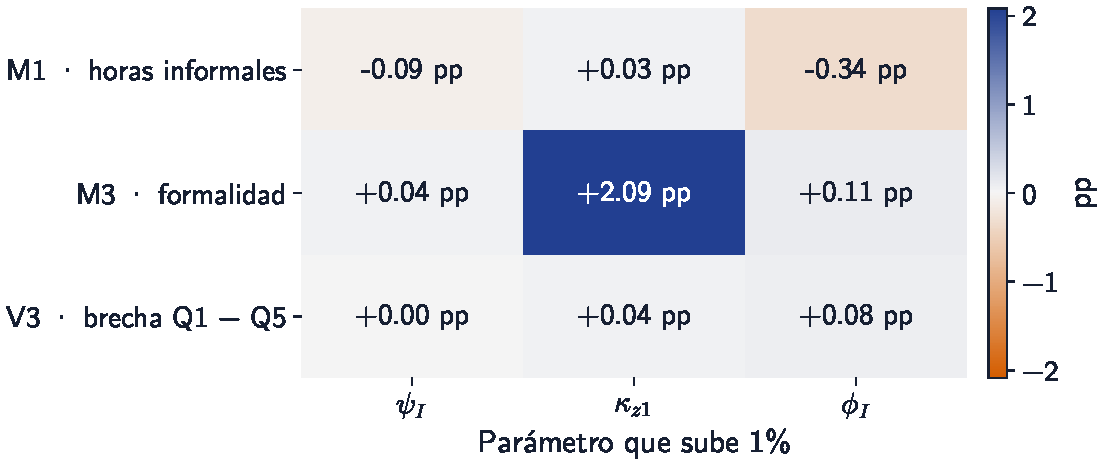
\includegraphics[width=\linewidth,height=5.6cm,keepaspectratio]{../code/figures/moment_sensitivity_map.pdf}
\figurenote{Cambio de cada momento si un parámetro sube 1\,\%, sin recalibrar; equilibrio parcial.}
\end{columns}
\end{frame}

% ===== Anexo: brecha V3 por elasticidad informal =====
\begin{frame}[label=av3]{A11. La brecha Q1$-$Q5 sube con $\phi_I$, \orange{pero sigue lejos del dato}}
\centering
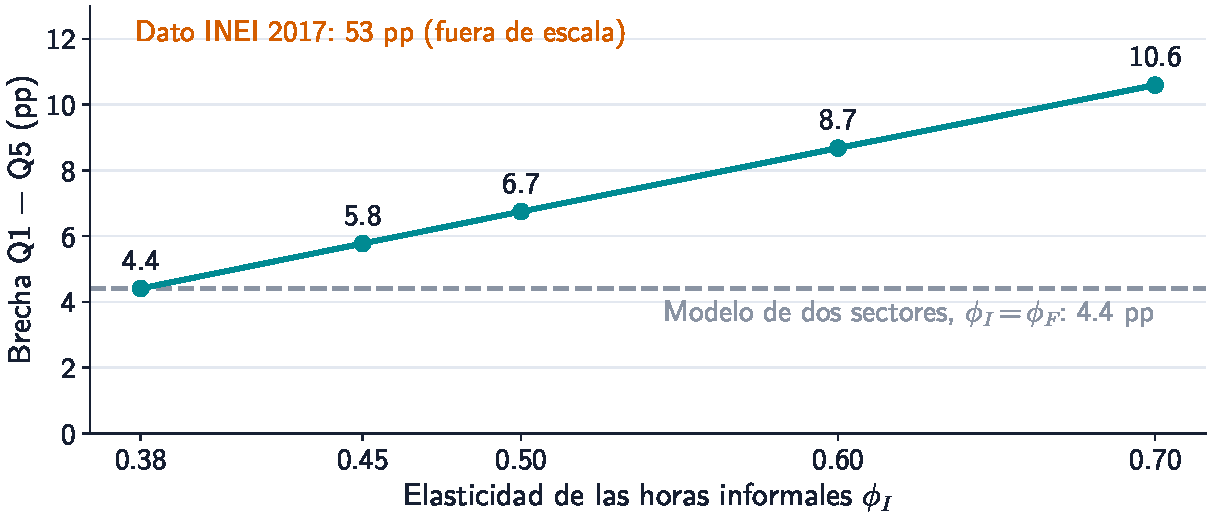
\includegraphics[width=\linewidth,height=6.4cm,keepaspectratio]{../code/figures/wealth_gap_by_phi.pdf}
\figurenote{Calibrado, equilibrio parcial; M1 y M3 fijos en cada punto (\hyperlink{a6}{anexo A10}; metas y validaciones: \hyperlink{amom}{anexo A9}). Brecha: fracción de horas informales del quintil de riqueza más bajo menos la del más alto.
Que no alcance el dato sugiere otro margen: entrar o salir de la informalidad (margen extensivo).}
\end{frame}

% ===== Anexo: formas de la barrera =====
\begin{frame}[label=aforms]{A12. Cambiar la forma de la barrera \teal{no cambia el resultado}}
\centering
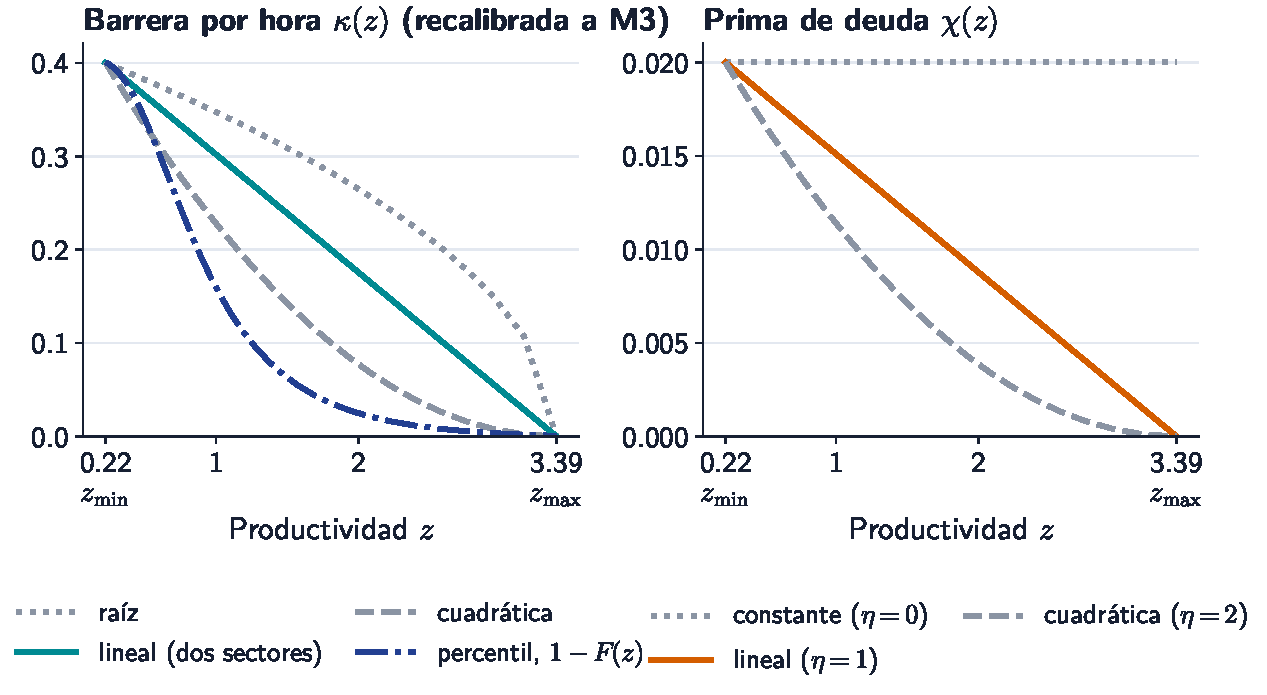
\includegraphics[width=\linewidth,height=4.5cm,keepaspectratio]{../code/figures/barrier_forms.pdf}
\par\vspace{2mm}
\begin{columns}[T,onlytextwidth]
\column{.48\textwidth}
\footnotesize\textbf{Barrera:} recalibrada a M3, $\kappa_{z1}$ queda en \KappaRangeShapes{} y la brecha Q1$-$Q5 en \VThreeKappaRangeBase{} pp; por percentil ($F$: distribución de $z$), \VThreePctBasePP{} pp.
Todas coinciden en $z_{\min}$ y $z_{\max}$, donde se mide M3, y $\kappa$ depende solo de $z$.
\column{.48\textwidth}
\footnotesize\textbf{Prima de deuda:} no entra en la FOC de horas; actúa a través de $V_a$, así que su forma solo se puede evaluar en equilibrio general (\hyperlink{a7}{anexo A13}).
\end{columns}
\vspace{3mm}
\begin{columns}[T,onlytextwidth]
\column{.48\textwidth}
\labeltext{Justificación de la forma}
Es la más simple que decrece en $z$ con un solo parámetro. $\kappa$ es una cuña por hora formal (trámites, requisitos): De Soto (1986) motiva las barreras.
\column{.48\textwidth}
\labeltext{\color{Orange}Su límite}
$z_{\min}$ y $z_{\max}$ son los extremos de la grilla de $z$: ampliarla cambia $w(z)$. La forma por percentil, $\kappa_0[1-F(z)]$, no depende de la grilla.
\end{columns}
\end{frame}

% ===== A7 =====
\begin{frame}[label=a7]{A13. \teal{Robustez}: forma de las cuñas y rendimiento informal de $z$}
\small
\renewcommand{\arraystretch}{1.35}
\begin{tabular}{@{}p{50mm}p{48mm}p{62mm}@{}}
\toprule
\textbf{Cambio} & \textbf{Evaluación} & \textbf{Brecha Q1$-$Q5}\\
\midrule
$\kappa(z)$ en raíz o cuadrática & recalibrada a M1 y M3 & \VThreeKappaRangeBase{} pp con $\phi$ común; \VThreeKappaRangeHigh{} pp con $\phi_I=\PhiHigh$\\
\ifnum\GeKappaAvailable=1
$\kappa(z)$ en raíz o cuadrática & equilibrio general, $\phi$ común & \GeKappaVThreeRange{} pp (lineal: \GeVThreeBaseTwoPP)\\
\fi
$\kappa(z)$ por percentil, $\kappa_0[1-F(z)]$ & recalibrada a M1 y M3 & \VThreePctBasePP{} pp con $\phi$ común; \VThreePctHighPP{} pp con $\phi_I=\PhiHigh$\\
$\nu_I=1$: ingreso informal proporcional a $z$ & recalibrado a M1 y M3 & \VThreeNuOnePP{} pp con $\phi$ común ($\kappa_{z1}=\KappaNuOne$); con $\phi_I=\PhiHigh$ se toca el tope de horas\\
Forma de $\chi(z)$: constante o cuadrática & no entra en la FOC de horas & solo cambia $V_a$: requiere equilibrio general\\
\bottomrule
\end{tabular}\par
\vspace{4mm}
{\footnotesize Salvo la fila de equilibrio general: equilibrio parcial con $V_a$, $g$ y precios del modelo de dos sectores. En equilibrio general, con el solver del modelo de dos sectores: $\phi_I=\PhiMid$ y $\PhiHigh$ aún no convergen; $\nu_I=1$ y otras formas de $\chi$, pendientes.}
\end{frame}

% ===== A8 =====
\begin{frame}[label=a8]{A14. Formalidad por educación: \orange{una cuña por hora no alcanza el gradiente}}
\centering
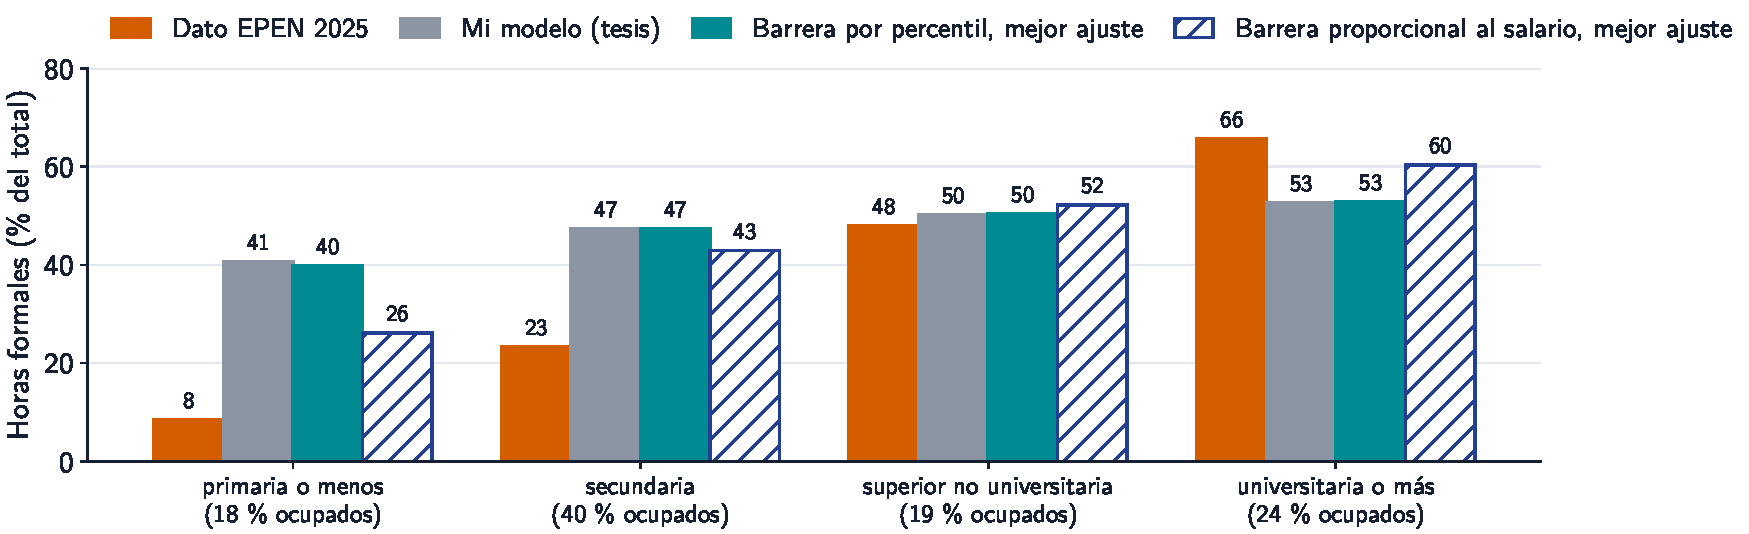
\includegraphics[width=\linewidth,height=5.1cm,keepaspectratio]{../code/figures/education_formality.pdf}
\par\vspace{1mm}
\raggedright
\begin{columns}[T,onlytextwidth]
\column{.48\textwidth}
\footnotesize\textbf{El límite del margen de horas.} Con $\phi$ común, $\ell_F/\ell_I\propto(R_F/R_I)^{\phi_F}$.
De primaria a universitaria los odds de horas formales suben \EduOddsData{} veces en el dato y \EduOddsModel{} en el modelo.
Para lograrlo, $R_F/R_I$ tendría que cambiar unas \EduRequiredRatio{} veces.
\column{.48\textwidth}
\footnotesize\textbf{Mejor ajuste a los 4 grupos} (M1 fijo).
Barrera decreciente: $R_F(z_{\min})>0$ topa su nivel; brecha \VSixPercentile{} pp.
Barrera proporcional al salario: \VSixAdValorem{} pp, pero cobra \AdValoremMedianPercent\,\% del salario formal mediano y lleva $\psi_I$ a \AdValoremPsiI.
\end{columns}
\figurenote{Calibrado, equilibrio parcial. Grupos asignados a tramos de la distribución de $z$ con su peso en la EPEN; un nodo que cruza un corte se reparte por masa. Dato de V6: \VSixData{} pp. Sugiere un margen extensivo (acceso a un empleo formal).}
\end{frame}

% ===== A9 =====
\begin{frame}[label=a9]{A15. \teal{Referencias} y fuentes de datos}
\scriptsize
\setlength{\parskip}{1.2mm}
\href{https://doi.org/10.1093/restud/rdab002}{Achdou, Y., Han, J., Lasry, J.-M., Lions, P.-L. y Moll, B. (2022)}. Income and wealth distribution in macroeconomics: a continuous-time approach. \textit{Review of Economic Studies}, 89(1), 45--86.

\href{https://doi.org/10.2307/2118417}{Aiyagari, S. R. (1994)}. Uninsured idiosyncratic risk and aggregate saving. \textit{Quarterly Journal of Economics}, 109(3), 659--684.

\href{https://ideas.repec.org/p/rbp/wpaper/2012-017.html}{Céspedes, N. y Rendón, S. (2012)}. La elasticidad de oferta laboral de Frisch en economías con alta movilidad laboral. BCRP, Documento de Trabajo 2012-017.

De Soto, H. (1986). \textit{El otro sendero: la revolución informal}. Lima: El Barranco.

\href{https://ideas.repec.org/p/rbp/wpaper/2024-005.html}{Galindo, H., Ledesma, A., Yépez, L. y Salinas, C. (2024)}. Informality and wealth distribution: a heterogeneous agent model. BCRP, Documento de Trabajo 2024-005.

\href{https://doi.org/10.1016/0165-1889(93)90024-M}{Huggett, M. (1993)}. The risk-free rate in heterogeneous-agent incomplete-insurance economies. \textit{Journal of Economic Dynamics and Control}, 17(5--6), 953--969.

INEI (2018). \textit{Perú: evolución de los indicadores de empleo e ingresos por departamento, 2007--2017}. Lima: INEI.

INEI (2022). \textit{Perú: evolución de los indicadores de empleo e ingresos por departamento, 2007--2021}. Lima: INEI.

\href{https://doi.org/10.1111/twec.12480}{Loayza, N. (2016)}. Informality in the process of development and growth. \textit{The World Economy}, 39(12), 1856--1916.

\href{https://doi.org/10.1257/aer.20121110}{Meghir, C., Narita, R. y Robin, J.-M. (2015)}. Wages and informality in developing countries. \textit{American Economic Review}, 105(4), 1509--1546.

\href{https://doi.org/10.1596/978-0-8213-7092-6}{Perry, G. E., Maloney, W. F., Arias, O. S., Fajnzylber, P., Mason, A. D. y Saavedra-Chanduvi, J. (2007)}. \textit{Informality: Exit and Exclusion}. Washington, DC: World Bank.

\href{https://doi.org/10.1016/j.red.2005.11.002}{Pijoan-Mas, J. (2006)}. Precautionary savings or working longer hours? \textit{Review of Economic Dynamics}, 9(2), 326--352.

\textbf{Fuentes de datos.} INEI: Encuesta Nacional de Hogares (ENAHO) 2015--2019 y Encuesta Permanente de Empleo Nacional (EPEN) 2025, microdatos de procesamiento propio; ENAHO 2021--2023, cálculo propio; Cuenta Satélite de la Economía Informal.
Banco Mundial: World Development Indicators, índice de Gini (SI.POV.GINI), Perú 2024.
\end{frame}

\begin{frame}[label=aasset]{A16. El interés \teal{equilibra ahorro y demanda de capital}}
\begin{columns}[T,onlytextwidth]
\column{.62\textwidth}
\centering
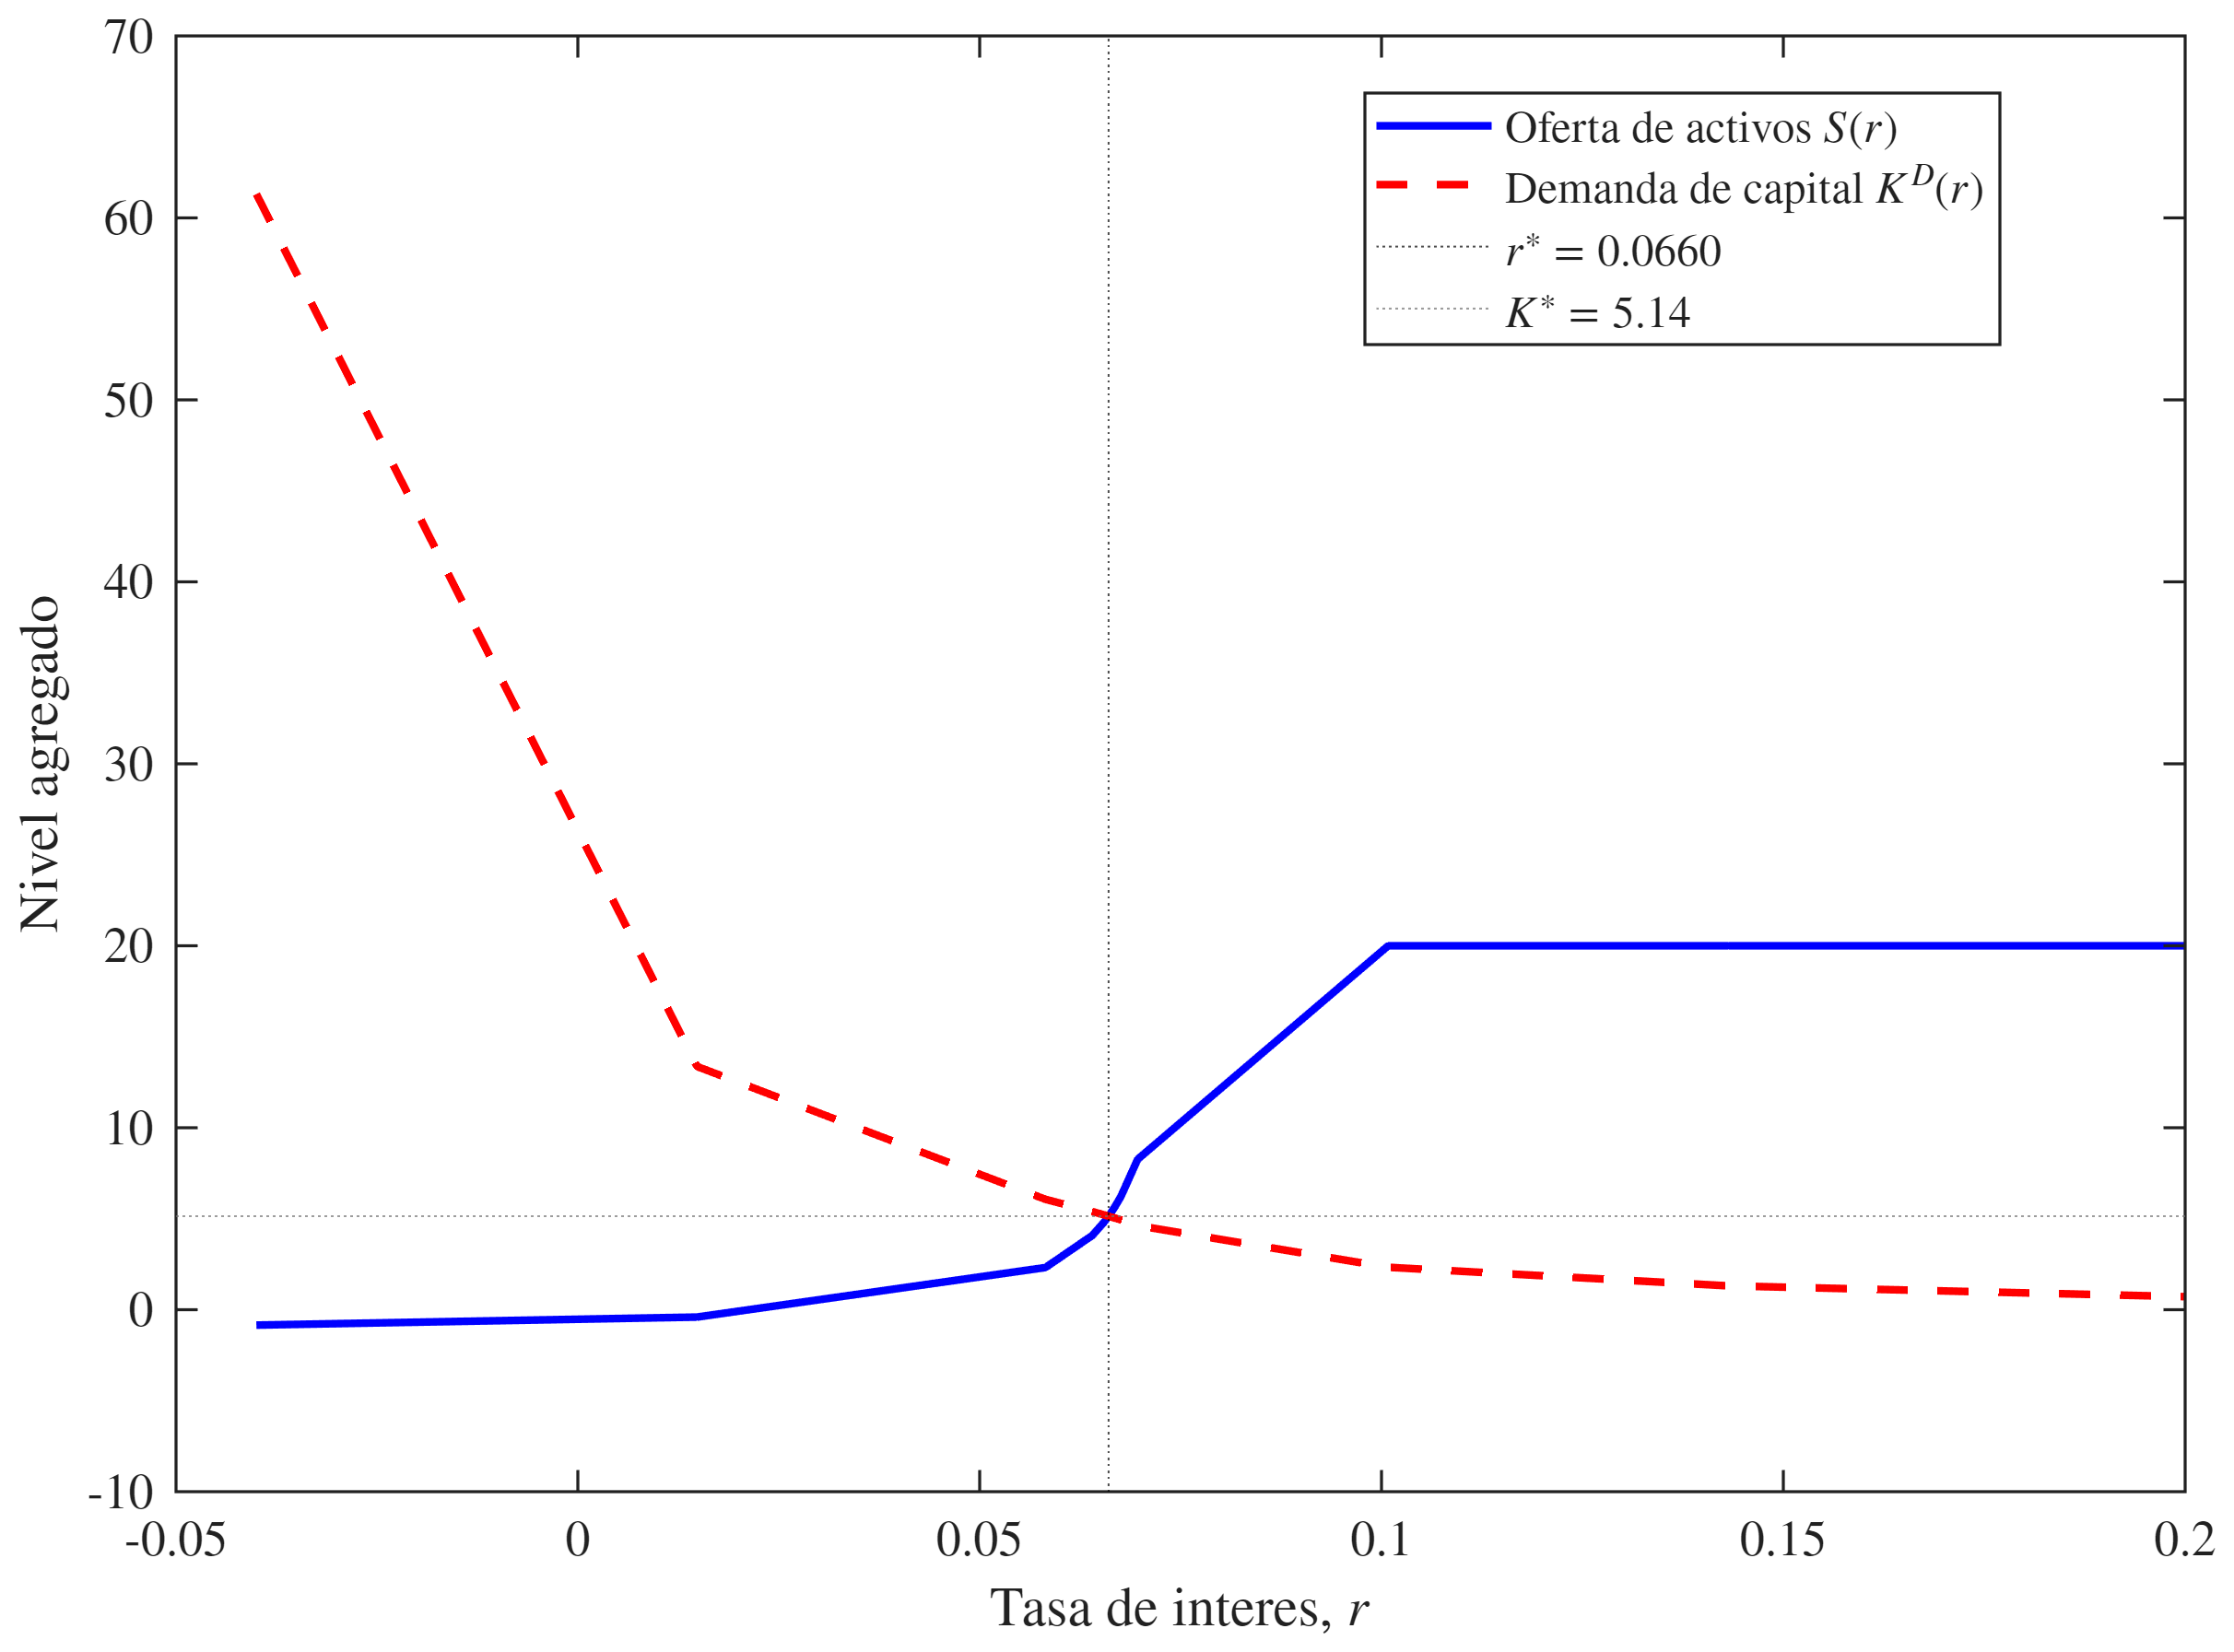
\includegraphics[width=\linewidth,height=6.2cm,keepaspectratio]{figures/base_model/moll_equilibrium_asset_market_matlab.png}
\column{.34\textwidth}
\labeltext{Dos decisiones agregadas}
$S(r)$: activos de los hogares.\par\vspace{3mm}
$K^D(r)=K_F+K_I$: capital de las firmas.\par\vspace{3mm}
En equilibrio coinciden.\par\vspace{3mm}
La línea une puntos calculados con distintas tasas de interés. No es tiempo.
\end{columns}
\figurenote{Figura histórica del modelo de dos sectores en MATLAB; procedencia en \texttt{figures/base\_model/PROCEDENCIA.md}. El tramo plano refleja el límite superior de la grilla de activos. Cierre de todos los mercados: \hyperlink{aeq}{anexo A5}.}
\end{frame}

\begin{frame}[label=aresult]{A17. Composición de horas: \teal{definiciones y condiciones}}
\labeltext{A una misma productividad laboral individual $z$}
\[
\frac{\ell_I}{\ell_F}=\frac{(R_I/\psi_I)^{\phi_I}}{(R_F/\psi_F)^{\phi_F}}\;V_a^{\,\phi_I-\phi_F}
\quad\Longrightarrow\quad
\frac{\partial\ln(\ell_I/\ell_F)}{\partial\ln V_a}=\phi_I-\phi_F
\]
\begin{columns}[T,onlytextwidth]
\column{.47\textwidth}
\panel{Pale}{\linewidth}{\labeltext{\color{Gray}Modelo de dos sectores: $\phi_I=\phi_F$}
$V_a$ se cancela: la fracción informal $s_I=\ell_I/(\ell_F+\ell_I)$ no depende de $a$ a igual $z$.
La barrera $\kappa(z)$ permanece en $R_F$: cambia el nivel del reparto, pero no depende directamente de $a$.}
\column{.47\textwidth}
\panel{PaleTeal}{\linewidth}{\labeltext{\color{Teal}Sensibilidad: $\phi_I>\phi_F$}
\[
\frac{\partial s_I}{\partial V_a}=s_I(1-s_I)\,\frac{\phi_I-\phi_F}{V_a}>0
\]
Si $V_a$ baja con $a$: más pobre $\Rightarrow$ más informal.}
\end{columns}
\vspace{3mm}
{\footnotesize\textbf{Condiciones:} (i) horas positivas y $\ell_F+\ell_I<\bar H$; (ii) $R_F(z),R_I(z)>0$, independientes de $a$, y $V_a,\phi_s,\psi_s>0$; (iii) $V_a$ decreciente en $a$: verificado en la grilla, no demostrado.
\par\vspace{2mm}\textbf{Comparación con el modelo de dos sectores:} recalibración en \hyperlink{a6}{A10}; aumento de V3 en \hyperlink{av3}{A11}.}
\end{frame}

\end{document}
